\documentclass[xcolor=dvipsnames,aspectratio=169,t]{beamer}
  % t means frames are vertically centered to the top
\usepackage{slides-header}
\title{Applications to Computer Graphics}
%% TODO: Re-do the graphics from a Jupyter Notebook so that the pictures can be made as vector images, and the examples can easily be changed.

\begin{document}
\maketitle

\begin{frame}{Applications of Linear Algebra to Computer Graphics}
\begin{columns}[T]

\column{0.5\tw}

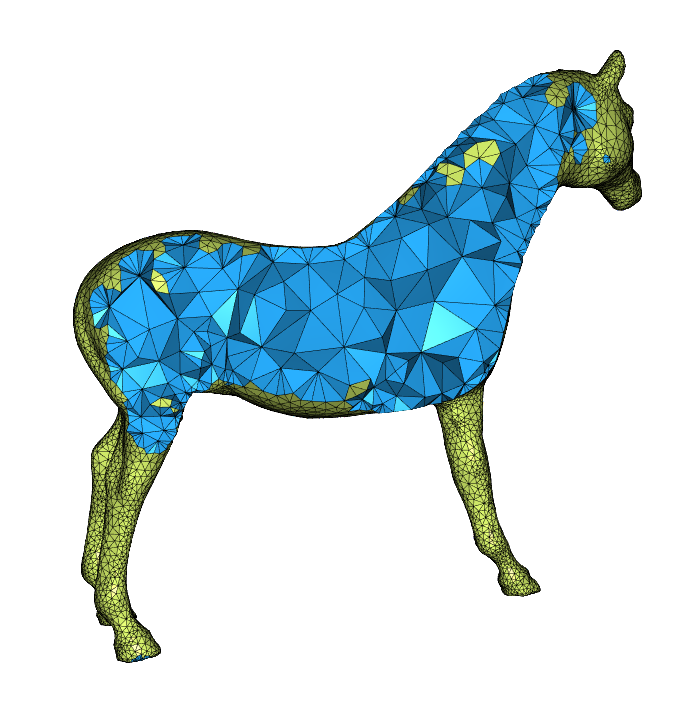
\includegraphics[width=0.8\tw]{images/fig-horse-triangular.png}

{\tiny \href{https://www.cg.tu-berlin.de/research/projects/harmonic-triangulations/}{\alert{https://www.cg.tu-berlin.de/research/projects/harmonic-triangulations/}}}

\column{0.5\tw}


\includegraphics[width=0.9\tw]{images/fig-yoda.jpg}

{\tiny Image Credit: Star Wars low poly portraits, designed by Vladan Filipovic}

\bs

\colorb{Let's examine some ways to manipulate and display graphical images using matrices.}

\end{columns}

\end{frame}

\begin{frame}{Scaling One Triangle}

Consider one triangular piece. If we want to scale the triangle by a factor of three, then we apply the transformation
\[ S: \mathbb{R}^2 \to \mathbb{R}^2: \mathbf{x} \mapsto \begin{bmatrix} 3 & 0 \\ 0 & 3 \end{bmatrix} \mathbf{x} .\]

\begin{columns}[T]

\column{0.5\tw}

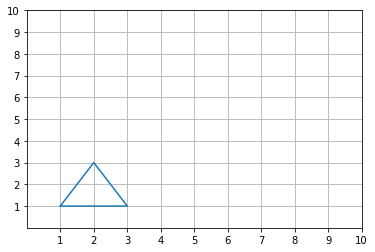
\includegraphics[width=0.9\tw]{images/fig-triangle-start.png}

\column{0.5\tw}

We have:
\[ \begin{bmatrix} 3 & 0 \\ 0 & 3 \end{bmatrix} \begin{bmatrix} 1 \\ 1 \end{bmatrix} = \begin{bmatrix} 3 \\ 3 \end{bmatrix}\] 

\[ \begin{bmatrix} 3 & 0 \\ 0 & 3 \end{bmatrix} \begin{bmatrix} 3 \\ 1 \end{bmatrix} =  \begin{bmatrix} 9 \\ 3 \end{bmatrix} \] 


\[ \begin{bmatrix} 3 & 0 \\ 0 & 3 \end{bmatrix} \begin{bmatrix} 2 \\ 3 \end{bmatrix} =  \begin{bmatrix} 6 \\ 9 \end{bmatrix}\]

\end{columns}

\end{frame}

\begin{frame}{Vertical Scaling}  % would be nice to have a shearing example

If we would like to vertically scale the triangle by a factor of 2, we have

\[ V: \mathbb{R}^2 \to \mathbb{R}^2: \mathbf{x} \mapsto \begin{bmatrix} 1 & 0 \\ 0 & 2 \end{bmatrix} \mathbf{x} .\]

\begin{columns}[T]

\column{0.5\tw}

We have:
\[ \begin{bmatrix} 1 & 0 \\ 0 & 2 \end{bmatrix} \begin{bmatrix} 1 \\ 1 \end{bmatrix} = \begin{bmatrix} 1 \\ 2 \end{bmatrix} \]
\[ \begin{bmatrix} 1 & 0 \\ 0 & 2 \end{bmatrix} \begin{bmatrix} 3 \\ 1 \end{bmatrix} =  \begin{bmatrix} 3 \\ 2 \end{bmatrix} \]
 \[ \begin{bmatrix} 1 & 0 \\ 0 & 2 \end{bmatrix} \begin{bmatrix} 2 \\ 3 \end{bmatrix} =  \begin{bmatrix} 2 \\ 6 \end{bmatrix} \]

\column{0.5\tw}

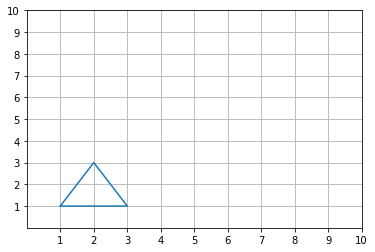
\includegraphics[width=0.95\tw]{images/fig-triangle-start.png}

\end{columns}

\end{frame}

\begin{frame}{Rotation}

\begin{columns}[T]

\column{0.6\tw}

If we would like to rotate the triangle counter-clockwise by an angle of $\theta$ around the origin, we have
\[ R: \mathbb{R}^2 \to \mathbb{R}^2: \mathbf{x} \mapsto \begin{bmatrix} \cos{\theta} & -\sin{\theta} \\ \sin{\theta} & \cos{\theta} \end{bmatrix} \mathbf{x} .\]

For example a counterclockwise rotation by $\theta = \frac{3 \pi}{2}$ would be given by
\[ R: \mathbb{R}^2 \to \mathbb{R}^2: \mathbf{x} \mapsto \begin{bmatrix} \cos{\frac{3 \pi}{2}} & -\sin{\frac{3 \pi}{2}} \\ \sin{\frac{3 \pi}{2}} & \cos{\frac{3 \pi}{2}} \end{bmatrix} \mathbf{x} = \begin{bmatrix} 0 & 1 \\ -1 & 0 \end{bmatrix} \mathbf{x}.\]

\column{0.4\tw}

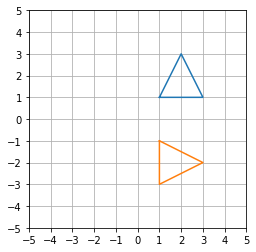
\includegraphics[width=0.8\tw]{images/fig-triangle-rotate.png}

\end{columns}

We have:

\[ \begin{bmatrix} 0 & 1 \\ -1 & 0 \end{bmatrix} \begin{bmatrix} 1 \\ 1 \end{bmatrix} = \begin{bmatrix} 1 \\ -1 \end{bmatrix} , \ \   \begin{bmatrix} 0 & 1 \\ -1 & 0 \end{bmatrix} \begin{bmatrix} 3 \\ 1 \end{bmatrix} =  \begin{bmatrix} 1 \\ -3 \end{bmatrix} , \ \  \begin{bmatrix} 0 & 1 \\ -1 & 0 \end{bmatrix} \begin{bmatrix} 2 \\ 3 \end{bmatrix} =  \begin{bmatrix} 3 \\ -2 \end{bmatrix} \]


\end{frame}

\begin{frame}{Composing Maps}
  Imagine we want to apply three transformations to the triangle in the following order:
  \bb
  \ii Scale the triangle by a factor of three.
  \ii Then vertically scale by a factor of 2 (in vertical direction only).
  \ii Finally rotate counter-clockwise around the origin by $\theta = 270^{\circ}=\frac{3 \pi}{2}$ radians.
  \ee

  \onslide*<2>{
  \begin{columns}[T]

  \column{0.25\tw}

  First apply the scaling matrix using matrix $S$:

  \[  \begin{bmatrix} 3 & 0 \\ 0 & 3 \end{bmatrix} \begin{bmatrix}1 \\ 1 \end{bmatrix} = \colorb{\begin{bmatrix} 3 \\ 3 \end{bmatrix}} .\]

  \column{0.25\tw}

  Then apply the vertical scaling using $V$:

  \[ \begin{bmatrix} 1 & 0 \\ 0 & 2 \end{bmatrix} \colorb{ \begin{bmatrix} 3 \\ 3 \end{bmatrix}} = \alert{\begin{bmatrix} 3 \\ 6 \end{bmatrix}}.\]

  \column{0.5\tw}

  Finally, we rotate this result counter-clockwise by $\theta = \frac{3 \pi}{2}$ using $R$:

  \[ \begin{bmatrix} \cos{\left( \frac{3 \pi}{2} \right)} & -\sin{\left( \frac{3 \pi}{2} \right)} \\ \sin{\left( \frac{3 \pi}{2} \right)} & \cos{\left( \frac{3 \pi}{2} \right)} \end{bmatrix} \alert{ \begin{bmatrix} 3 \\ 6 \end{bmatrix} } = \colorg{ \begin{bmatrix} 6 \\ -3 \end{bmatrix} }.\]

  \end{columns}

  \bbox
  {\small
  The image under the composition of these three transformations is  $R \bigg( V \big( S (\x) \big) \bigg) = (RVS) (\x)$}
  \ebox
  }
  \onslide*<3->{
  \begin{columns}[T]

  \column{0.6\tw}

  \[ M: \mathbb{R}^2 \to \mathbb{R}^2: \mathbf{x} \mapsto RVS \mathbf{x} .\]

  where
  \[ RVS =  \begin{bmatrix} \cos{\left( \frac{3 \pi}{2} \right)} & -\sin{\left( \frac{3 \pi}{2} \right)} \\ \sin{\left( \frac{3 \pi}{2} \right)} & \cos{\left( \frac{3 \pi}{2} \right)} \end{bmatrix} \begin{bmatrix} 1 & 0 \\ 0 & 2 \end{bmatrix} \begin{bmatrix} 3 & 0 \\ 0 & 3 \end{bmatrix}  = 
  \begin{bmatrix} 0 & 6 \\ -3 & 0 \end{bmatrix}.\]

  Thus we have
  \[ \begin{bmatrix} 0 & 6 \\ -3 & 0 \end{bmatrix} \begin{bmatrix} 1 \\ 1 \end{bmatrix} = \begin{bmatrix} 6 \\ -3 \end{bmatrix} \]

  \column{0.4\tw}

  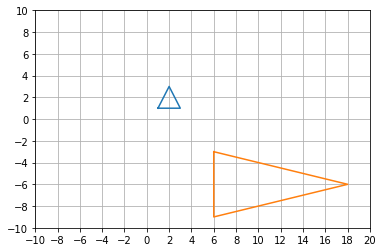
\includegraphics[width=0.9\tw]{images/fig-triangle-combo1.png}

  \end{columns}
  }
\end{frame}

\begin{frame}{Composing Linear Transformations}
  \bbox
  The composition of linear transformations with associated matrices $A$, $B$, and $C$ in the following order:
  \bb
  \item first apply transformation given by matrix $A$,
  \item then apply transformation given by matrix $B$, and 
  \item finally apply transformation given by matrix $C$
  \ee
  is equivalent to the linear transformation with associated matrix given by %the product
  $CBA$. 
  \ebox

\colorb{Note we can extend this idea to compose any number of linear transformations. }

\end{frame}

\begin{frame}{Translations}

To translate the vertex of the triangle at $(1,1)$  to the left by 2 units and up by 3 units, \alert{we add vectors}:

\[ \begin{bmatrix} 1 \\ 1\end{bmatrix} + \begin{bmatrix} -2 \\ 3 \end{bmatrix} = \begin{bmatrix} -1 \\ 4 \end{bmatrix}\]

\begin{columns}

\column{0.5\tw}

Doing the same for the other two vertices, we have

\[ \begin{bmatrix} 3 \\ 1\end{bmatrix} + \begin{bmatrix} -2 \\ 3 \end{bmatrix} = \begin{bmatrix} 1 \\ 4 \end{bmatrix} \qquad
\begin{bmatrix} 2 \\ 3\end{bmatrix} + \begin{bmatrix} -2 \\ 3 \end{bmatrix} = \begin{bmatrix} 0 \\ 6 \end{bmatrix}.\]


\column{0.5\tw}

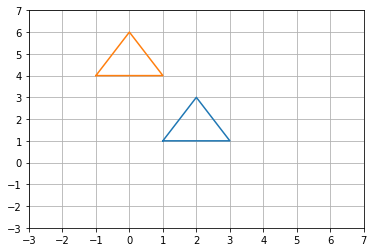
\includegraphics[width=0.9\tw]{images/fig-triangle-shift.png}

\end{columns}

\end{frame}

\begin{frame}{Homogeneous Coordinates}
  \bi
  \ii Operations such as shearing, scaling, rotations are \alert{linear transformations}.
  \bi
    \ii [$\circ$] These operations can be defined by \alert{matrix multiplication}.
  \ei
  \pause
  \ii \colorb{A translation is not a linear transformation}. We \colorb{add vectors rather than multiply}.
  \ii How can we compose translations with the other linear transformations if translation cannot be represented as matrix multiplication?
  \ei
  
  \pause
  \bbox
  One common way is to introduce \alert{homogeneous coordinates}:

  \bi
  \ii Each point $(x,y)$ in $\mathbb{R}^2$ can be identified with the point $(x,y,1)$ in $\mathbb{R}^3$.
  \ii We say $(x,y)$ has homogeneous coordinates $(x,y,1)$.
  \ei
  \ebox

\end{frame}

\begin{frame}{Homogeneous Coordinates}
  Now we can perform translation by matrix multiplication. For example, if we want to shift the point $(3,1)$ to the left by 2 units and up by the 3 units, then we have the product

  \[ \begin{bmatrix}1 & 0 & -2\\ 0 & 1 & 3 \\ 0 & 0 & 1\end{bmatrix} \begin{bmatrix}3 \\ 1\\ 1 \end{bmatrix} = \begin{bmatrix} 3-2 \\ 1+3 \\ 1 \end{bmatrix} = \begin{bmatrix}1\\4\\1 \end{bmatrix}\]
  \medskip

  \pause
  \bbox
  In general, if we want to translate by $h$ units in the horizontal direction and $k$ units in the vertical direction, using homogeneous coordinates we have:

  \[ \begin{bmatrix} 1 & 0 & h \\ 0 & 1 & k \\ 0 & 0 & 1 \end{bmatrix} \begin{bmatrix}x \\ y \\ 1 \end{bmatrix} = \begin{bmatrix} x+h \\ y+k \\ 1 \end{bmatrix}.\]
  \ebox
\end{frame}

\begin{frame}
  Let's perform a composition of three different transformations to the triangle in the following order:

  \bb
  \ii \alert{Scale the triangle by a factor of 3.}
  \ii \colorb{Rotate the triangle counter-clockwise around the origin by $\frac{\pi}{2}$.}
  \ii \colorg{Translate to the right by 5 units and down by 2 units.}
  \ee

  We have the following three matrices for the scaling \alert{$S$}, rotation \colorb{$R$}, and translation \colorg{$B$}, respectively,

\[ \alert{S = \begin{bmatrix} 3 & 0 & 0 \\ 0 & 3 & 0 \\ 0 & 0 & 1 \end{bmatrix}} \qquad
\colorb{R = \begin{bmatrix} \cos{\frac{\pi}{2}} & -\sin{\frac{\pi}{2}}& 0 \\ \sin{\frac{\pi}{2}} & \cos{\frac{\pi}{2}} & 0 \\ 0 & 0 & 1 \end{bmatrix} = \begin{bmatrix} 0 & -1 & 0 \\ 1 & 0 & 0 \\ 0 & 0 & 1 \end{bmatrix}} \qquad
\colorg{B = \begin{bmatrix} 1 & 0 & 5 \\ 0 & 1 & -2 \\ 0 & 0 & 1 \end{bmatrix}}.\]

  We can now compose all three maps by multiplying matrices:

\[\colorg{B}\colorb{R}\alert{S} =  \colorg{\begin{bmatrix} 1 & 0 & 5 \\ 0 & 1 & -2 \\ 0 & 0 & 1 \end{bmatrix}}
\colorb{\begin{bmatrix} 0 & -1 & 0 \\ 1 & 0 & 0 \\ 0 & 0 & 1 \end{bmatrix}}
\begin{bmatrix} 3 & 0 & 0 \\ 0 & 3 & 0 \\ 0 & 0 & 1 \end{bmatrix} = \begin{bmatrix} 0 & -3 & 5\\
3 & 0 & 2 \\ 0 & 0 & 1 \end{bmatrix}.\]
\end{frame}

\begin{frame}
\bb
\ii \alert{Scale the triangle by a factor of 3.}
\ii \colorb{Rotate the triangle counter-clockwise around the origin by $\frac{\pi}{2}$.}
\ii \colorg{Translate to the right by 5 units and down by 2 units.}
\ee

\begin{columns}[T]

\column{0.5\tw}
Then we have each vertex (given in homogeneous coordinates) mapped as follows

$$\begin{bmatrix} 0 & -3 & 5\\
3 & 0 & 2 \\ 0 & 0 & 1 \end{bmatrix} \begin{bmatrix} 1 \\ 1 \\ 1 \end{bmatrix} = \begin{bmatrix} 2 \\ 1 \\ 1 \end{bmatrix}$$

$$\begin{bmatrix} 0 & -3 & 5\\
3 & 0 & 2 \\ 0 & 0 & 1 \end{bmatrix} \begin{bmatrix} 3 \\ 1 \\ 1 \end{bmatrix} \mapsto \begin{bmatrix} 2 \\ 7 \\ 1 \end{bmatrix}$$

$$\begin{bmatrix} 0 & -3 & 5\\
3 & 0 & 2 \\ 0 & 0 & 1 \end{bmatrix} \begin{bmatrix} 2 \\ 3 \\ 1 \end{bmatrix} \mapsto \begin{bmatrix} -4 \\ 4 \\ 1 \end{bmatrix}.$$

\column{0.5\tw}

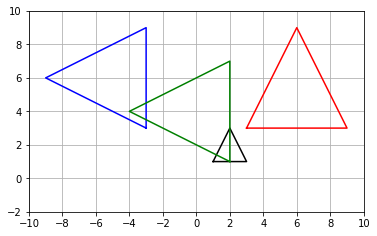
\includegraphics[width=0.9\tw]{images/fig-triangle-combo2.png}

\end{columns}

\end{frame}

\end{document}

